\subsubsection*{Zadanie~251.}
\begin{figure}[H]
    \centering
    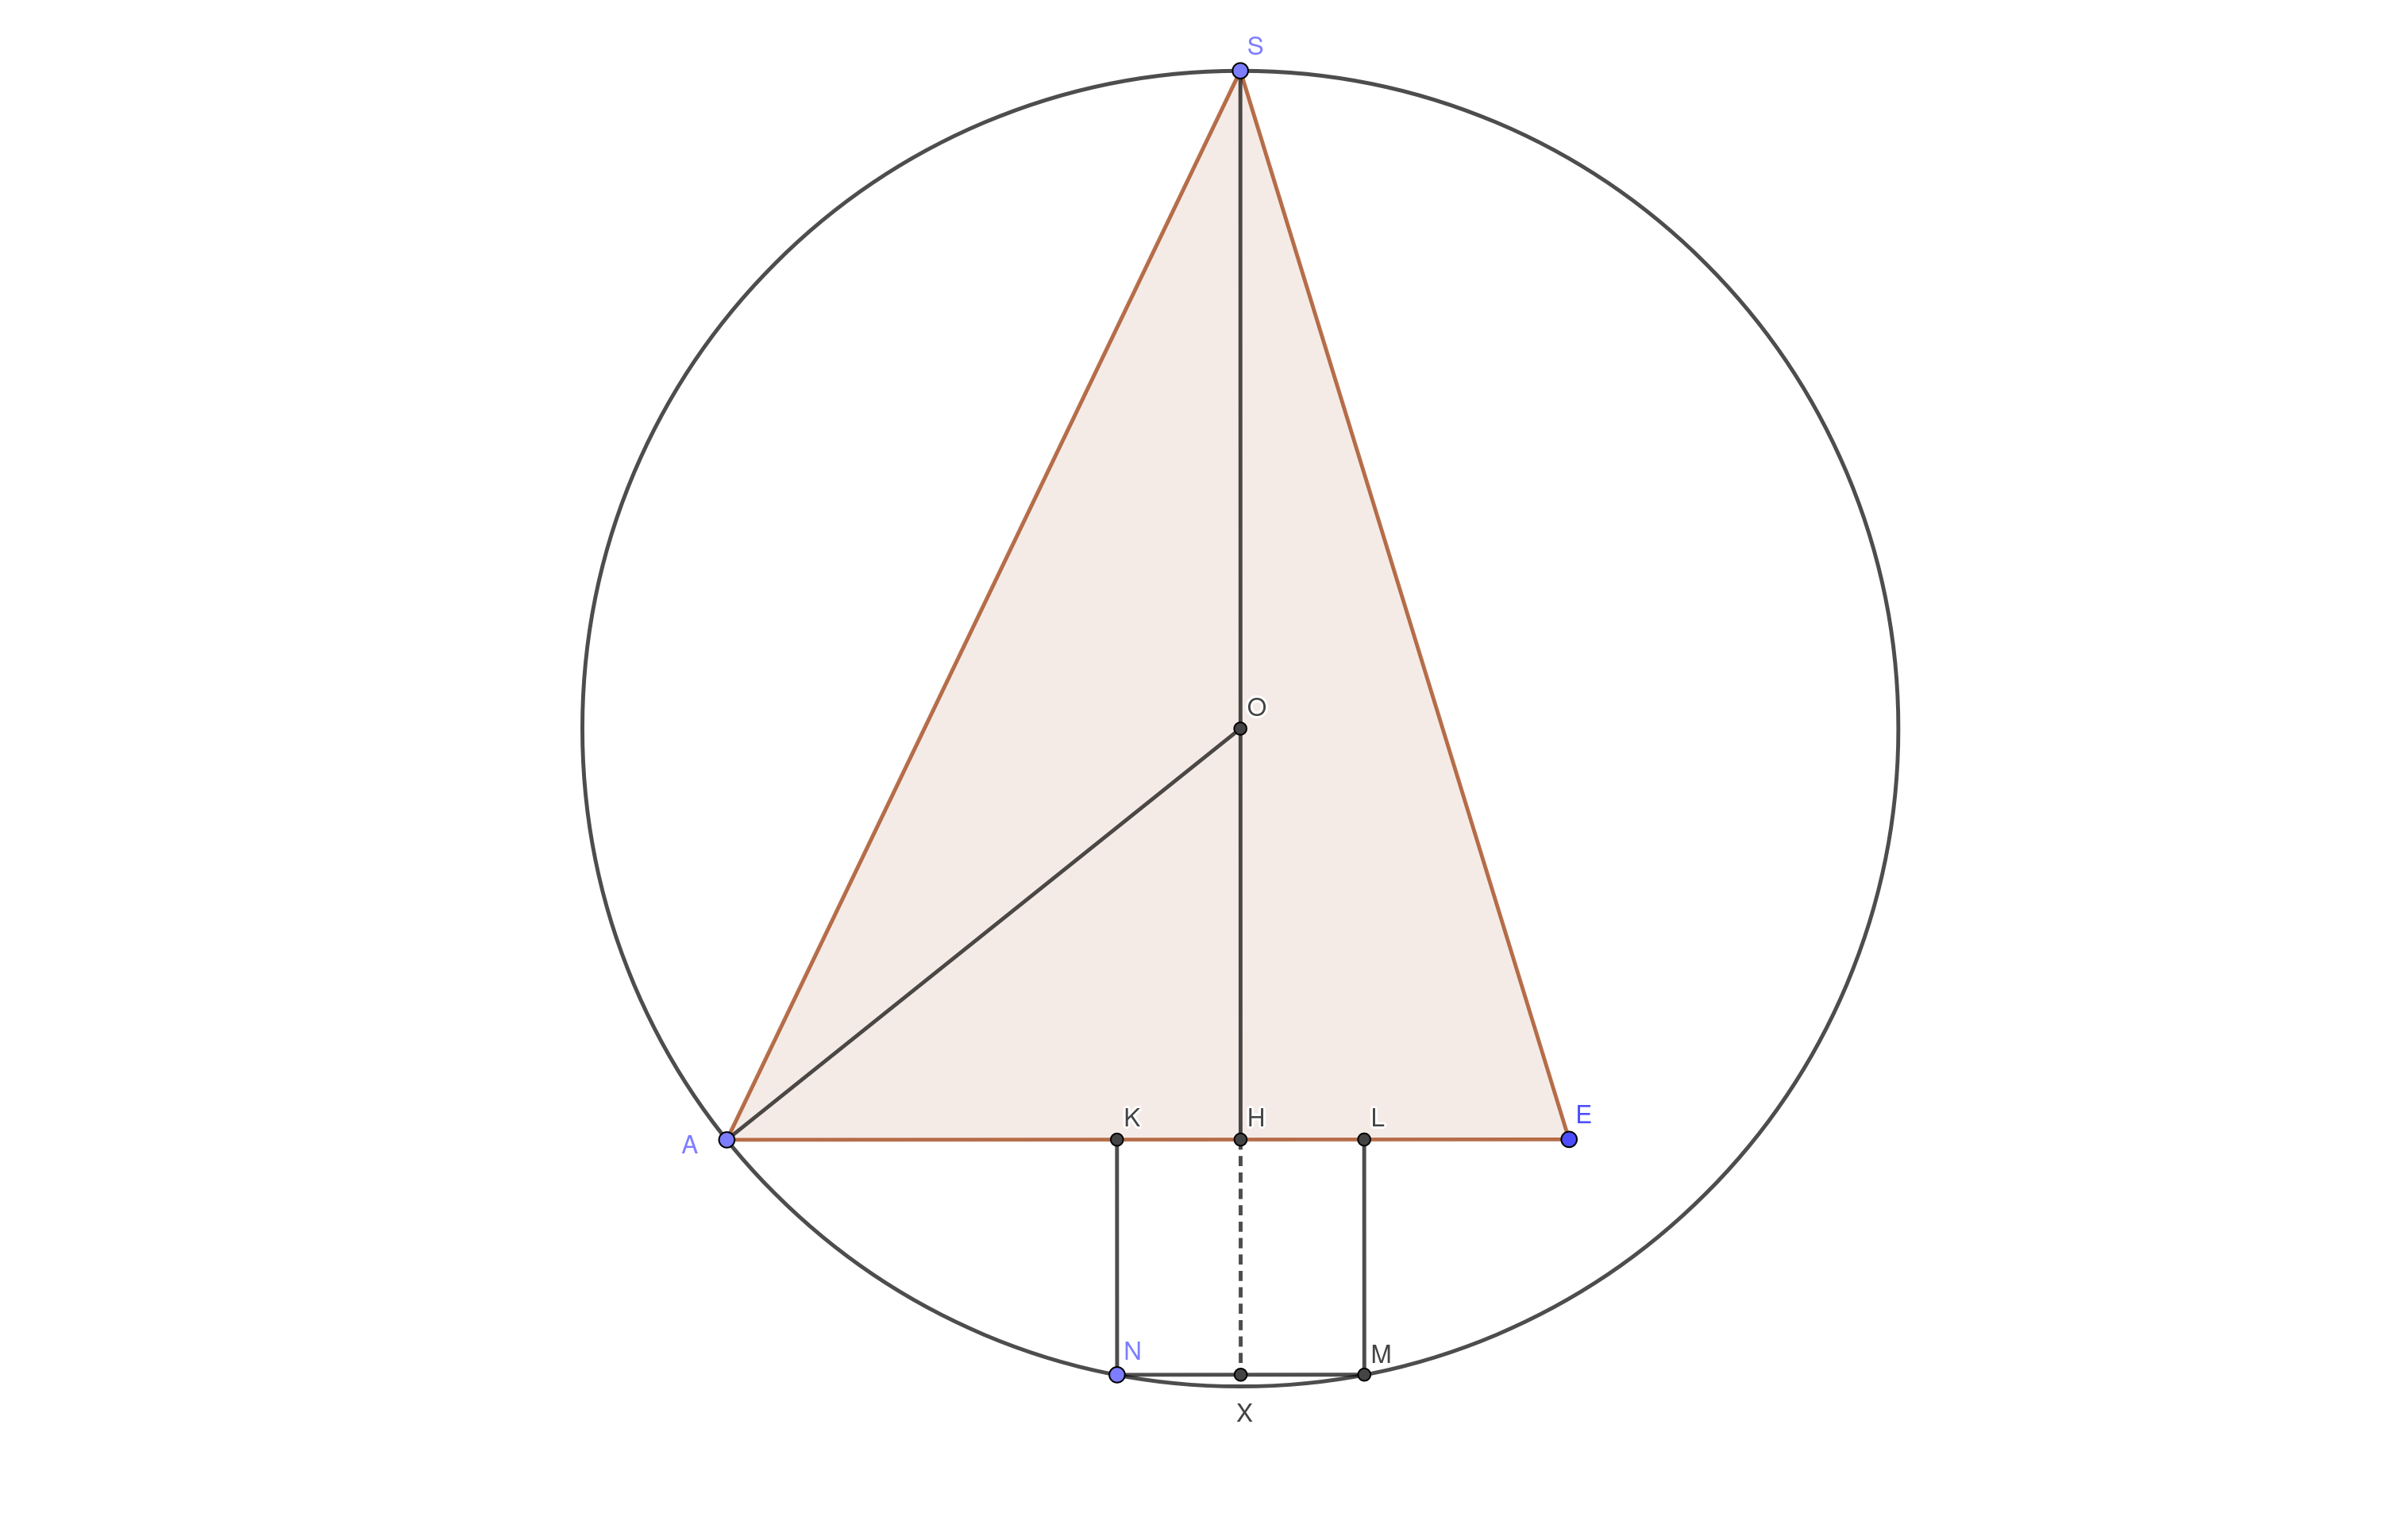
\includegraphics[width=\textwidth]{img/2021_03_02/251/space.png}
\end{figure}
\noindent
Zauważmy, że
\begin{gather*}
    SO = AO = R\\
    AO = \frac{\sqrt{5}}{1 + \sqrt{5}} \cdot h\\
    R = \frac{\sqrt{5}}{1 + \sqrt{5}} \cdot h\\
    h = \frac{1 + \sqrt{5}}{\sqrt{5}}R\\
    OH
    = h - R
    = \frac{1 + \sqrt{5}}{\sqrt{5}}R - R
    = \frac{R}{\sqrt{5}}
\end{gather*}
Z~twierdzenia Pitagorasa dla \(\triangle{SHA}\):
\begin{gather*}
    R^2 = \frac{R^2}{5} + \frac{a^2}{3}\\
    \frac{4}{5}R^2 = \frac{a^2}{3}\\
    R = \sqrt{\frac{5a^2}{12}} = \frac{a}{2}\sqrt{\frac{5}{3}}\\
    OH
    = \frac{R}{\sqrt{5}}
    = \frac{\frac{a}{2} \cdot \frac{\sqrt{5}}{\sqrt{3}}}{\sqrt{5}}
    = \frac{a}{2\sqrt{3}}
\end{gather*}
Oznaczmy przez \(p\) połowę długości przekątnej podstawy graniastosłupa, a~przez \(q\) oznaczmy jego wysokość. Z~twierdzenia Pitagorasa dla \(\triangle{OXM}\) mamy
\begin{gather*}
    \pars{\frac{a}{2\sqrt{3}} + q}^2 + p^2 = R^2\\
    \frac{a^2}{12} + q^2 + \frac{aq}{\sqrt{3}} + p^2 = \frac{5a^2}{12}\\
    q^2 + p^2 + \frac{aq}{\sqrt{3}} = \frac{a^2}{3}\\
    p^2 = \frac{a^2}{3} - \frac{aq}{\sqrt{3}} - q^2\\
    V\pars{q}
    = 2p^2q
    = \frac{2a^2q}{3} - \frac{2aq^2}{\sqrt{3}} - 2q^3 \qquad D = \open{0}{R\pars{1 - \frac{1}{\sqrt{5}}}} = \open{0}{\frac{a}{2}\sqrt{\frac{5}{3}}\pars{1 - \frac{1}{\sqrt{5}}}}\\
    V'\pars{q}
    = \frac{2a^2}{3} - \frac{4aq}{\sqrt{3}} - 6q^2\\
    -6q^2 - \frac{4aq}{\sqrt{3}} + \frac{2a^2}{3} = 0\\
    -3q^2 - \frac{2aq}{\sqrt{3}} + \frac{a^2}{3} = 0\\
    \Delta
    = \frac{4a^3}{3} + 4a^2
    = \frac{16}{3}a^2\\
    \sqrt{\Delta} = \frac{4a}{\sqrt{3}}\\
    q_1 = \frac{\frac{2a}{\sqrt{3}} - \frac{4a}{\sqrt{3}}}{-6}
    = \frac{a}{3\sqrt{3}} \in D\\
    D \not\ni q_2 < 0\\
\end{gather*}
Wykres znaku pochodnej:
\begin{gather*}
    \downparabola{q_2}{\frac{a}{3\sqrt{3}}}
\end{gather*}
Pochodna jest dodatnia w~przedziale \(\open{0}{\frac{a}{3\sqrt{3}}}\) i~ujemna w~przedziale \(\open{\frac{a}{3\sqrt{3}}}{\frac{a}{2}\sqrt{\frac{5}{3}}\pars{1 - \frac{1}{\sqrt{5}}}}\), a~dla \(q = \frac{a}{3\sqrt{3}}\) przyjmuje wartość \(0\). Oznacza to, że w~przedziale \(\open{0}{\frac{a}{3\sqrt{3}}}\) funkcja \(V\) jest rosnąca, a~w~przedziale \(\open{\frac{a}{3\sqrt{3}}}{\frac{a}{2}\sqrt{\frac{5}{3}}\pars{1 + \frac{1}{\sqrt{5}}}}\) jest malejąca, więc dla \(q = \frac{a}{3\sqrt{3}}\) przyjmuje globalną wartość największą:
\begin{equation*}
    V_\p{max}
    = V\pars{\frac{a}{3\sqrt{3}}}
    = \frac{2a^2q}{3} - \frac{2aq^2}{\sqrt{3}} - 2q^3
    = \frac{2a^3}{9\sqrt{3}} - \frac{2a^3}{27\sqrt{3}} - \frac{2a^3}{81\sqrt{3}}
    = \frac{18a^3 - 6a^3 - 2a^3}{81\sqrt{3}}
    = \frac{10a^3}{81\sqrt{3}}
\end{equation*}
Graniastosłup osiąga największą objętość równą \(\frac{10a^3}{81\sqrt{3}}\), kiedy jego wysokość wynosi \(\frac{a}{3\sqrt{3}}\)
\subsubsection*{Zadanie~252a).}
Rozważmy przekrój osiowy stożka:
\begin{mathfigure*}
    \coordinate (A) at (-3, 0);
    \coordinate (B) at (3, 0);
    \coordinate (C) at (0, 6);
    \coordinate (I) at (0, 1.85);
    \coordinate (E) at (1.66, 2.68);
    \coordinate (D) at (0, 0);
    \drawangle[Orange]{D--C--B};
    \drawangle*[RoyalBlue]{E--I--C}[\(\alpha\)];
    \drawangle*[RoyalBlue]{C--B--D}[\(\alpha\)];
    \draw (I) circle[radius=1.85];
    \draw (C) -- node[left]{\(h\)} (D);
    \draw (I) -- node[above, sloped]{\(r\)} (E);
    \path (I) -- node[left]{\(r\)} (D);
    \draw (A) -- node[pos=0.75, below]{\(R\)} (B) -- (C) -- node[above left]{\(\ell\)} cycle;
    \drawrightangle{B--D--C};
    \drawrightangle{C--E--I};
    \fillpoint*{A}[\(A\)][below left];
    \fillpoint*{B}[\(B\)][below right];
    \fillpoint*{C}[\(C\)][above];
    \fillpoint*{I}[\(I\)][below left];
    \fillpoint*{E}[\(E\)][above right];
    \fillpoint*{D}[\(D\)][below];
\end{mathfigure*}
\noindent
Zauważamy tu podobieństwo:
\begin{equation*}
    \triangle{CIE} \sim \triangle{CBD}
\end{equation*}
Zatem
\begin{gather*}
    \frac{R}{\ell} = \frac{r}{h - r}\\
    R\pars{h - r} = r\ell\\
    Rh - Rr = r\ell\\
    Rr + r\ell = Rh\\
    r\pars{R + \ell} = Rh\\
    r
    = \frac{Rh}{R + \ell}
\end{gather*}
Możemy teraz obliczyć objętości:
\begin{gather*}
    V_\p{stożka}
    = \frac{1}{3}\pi R^2h\\
    V_\p{kuli}
    = \frac{4}{3}\pi r^3
    = \frac{4}{3}\pi\pars{\frac{Rh}{R + \ell}}^3
    = \frac{4}{3}\pi \cdot \frac{R^3h^3}{\pars{R + \ell}^3}\\
    \frac{V_\p{stożka}}{V_\p{kuli}}
    = \frac{\frac{1}{\cancel{3}}\cancel{\pi}\cancel{R^2}\cancel{h}}{\frac{4}{\cancel{3}}\cancel{\pi} \cdot \frac{R^{\cancel{3}}h^{\cancel{3}^2}}{\pars{R + \ell}^3}}
    = \frac{1}{\frac{4Rh^2}{\pars{R + \ell}^3}}
    = \frac{\pars{R + \ell}^3}{4Rh^2}
\end{gather*}
Teraz możemy wyznaczyć pola powierzchni i~ich stosunek:
\begin{gather*}
    S_\p{stożka}
    = \pi R^2 + \pi R\ell
    = \pi R\pars{R + \ell}
    = \pi R\pars{R + \sqrt{R^2 + h^2}}\\
    S_\p{kuli}
    = 4\pi r^2
    = 4\pi\pars{\frac{Rh}{R + \ell}}^2
    = 4\pi \cdot \frac{R^2h^2}{\pars{R + \ell}^2}\\
    \frac{S_\p{stożka}}{S_\p{kuli}}
    = \frac{\cancel{\pi} \cancel{R}\pars{R + \ell}}{4\cancel{\pi} \cdot \frac{R^{\cancel{2}}h^2}{\pars{R + \ell}^2}}
    = \frac{R + \ell}{\frac{4Rh^2}{\pars{R + \ell}^2}}
    = \frac{\pars{R + \ell}^2\pars{R + \ell}}{4Rh^2}
    = \frac{\pars{R + \ell}^3}{4Rh^3}\\
    \frac{V_\p{stożka}}{V_\p{kuli}} = \frac{S_\p{stożka}}{S_\p{kuli}}
\end{gather*}
\qed
